\documentclass{beamer}
\usetheme{Warsaw}
\usepackage{nhtvslides}
\usepackage{amssymb}
\usepackage{amsmath}
\usepackage{graphicx}
\usepackage{epsfig}
\usepackage{subfigure}
\usepackage{listings}
\usepackage{natbib}
\usepackage{verbatim}
\usepackage{enumitem}
\usepackage[utf8]{inputenc}
\usepackage[T1]{fontenc}
\usepackage{listings}
\usepackage[font=small,labelfont=bf]{caption}
\lstset{language=ml}
\lstset{commentstyle=\textit}
\lstset{mathescape=true}
\lstset{backgroundcolor=,rulecolor=}
\lstset{frame=single}
\lstset{breaklines=true}
\lstset{basicstyle=\footnotesize\ttfamily}

\title{Binary information}

\title{Resource Entity Action: A Generalized Design Pattern for RTS games}

\author{
Mohamed Abbadi\and Francesco Di Giacomo\and Renzo Orsini\and\\
Aske Plaat \and Pieter Spronck \and Giuseppe Maggiore\\
E-mail: \{mabbadi,fdigiacomo,orsini\}@dais.unive.it,
\{a.plaat,p.spronck\}@uvt.nl,
maggiore.g@nhtv.nl
}

\institute{Universit\`a Ca' Foscari DAIS - Computer Science, Venice, Italy \\[1mm]
Tilburg University, Netherlands\\[1mm]
NHTV University of Applied Sciences, Breda, Netherlands\\[1mm]
}

\date{}

\begin{document}
\maketitle

\begin{frame}{Table of contents}
\tableofcontents
\end{frame}

\section{Introduction}
\begin{slide}{Introduction to the problem}{Encoding}{
\item Building real-time video-games, fast
\item Simple game definition through high level patterns
\item High performance through automated optimization
\item Save a lot of work, do not decrease quality
\item Especially important for serious/research games
}\end{slide}

\begin{slide}{Introduction to the problem}{Casanova so far}{
\item Declarative language
\item Centered on (real-time) games
\item Design philosophy: few and simple orthogonal concepts, all game-focused
\begin{itemize}
\item Game world, entities
\item Rules
\item Scripts
\end{itemize}
}\end{slide}

\begin{frame}[fragile]{Introduction to the problem}
\begin{lstlisting}
world BouncingBall = {
  Sprite   : Sprite
  Position : Vector2<m>
  Velocity : Vector2<m/s>

  rule Sprite.Position'(world:BouncingBall) = 
    world.Position
  rule Position'(world:BouncingBall, dt:float<s>) =
    world.Position + world.Velocity * dt
  rule Velocity'(world:BouncingBall, dt:float<s>) =
    world.Velocity - Vector2.UnitY * 9.81<m/s^2> * dt
}
\end{lstlisting}
\end{frame}

\begin{frame}[fragile]{Introduction to the problem}
\begin{lstlisting}
let world = 
  { Sprite = ...; Position = ...; Velocity = ... }

let main = return ()

let input = 
  [
    wait_key_press Keys.Escape => quit()
    wait_key_down Keys.Space  =>
      co{
        world.Position := Vector2.Zero
        world.Velocity := Vector2.Zero
        wait_key_up Keys.Space || wait 0.2<s>
      }
  ]
\end{lstlisting}
\end{frame}

\begin{slide}{Introduction to the problem}{Our current focus}{
\item RTS games
\item Their high relevance
\begin{itemize}
\item Large commercial adoption
\item Potential high impact outside entertainment
\end{itemize}
\item Their issues: such games are quite hard to build
}\end{slide}

\begin{slide}{Introduction to the problem}{Building RTS games}{
\item Traditional engines/software engineering
\item At most, reuse of the game core, plus restyling
\item Not flexible
\item Compared to other genres (FPS!), little code reuse
}\end{slide}

\section{Generalizing RTS games}
\begin{slide}{Generalizing RTS games}{Generalizing RTS games}{
\item Building a simple algebra for entities and resources
\item \textbf{Entities} - a container of resources and other attributes
\item \textbf{Resources} - a (usually sparse) vector
\item \textbf{Actions} - a (usually sparse) matrix of resources conversion
}\end{slide}

\begin{frame}[fragile]{Generalizing RTS games}
\begin{lstlisting}
Source $e$, targets $T = \left\lbrace t_{1},t_{2},...,t_{n}\right\rbrace$, action $A$ (a transformation matrix).

Each entity has resource vector $\mathbf{r_{i}}=\left(r_{i_{1}},r_{i_{2}},...,r_{i_{m}} \right)$

We compute $\mathbf{w_{e}} = \left(  w_{e_{1}},w_{e_{2}},...,w_{e_{m}} \right) = \mathbf{r_{s}} \times A \cdot dt$. 

We compute the new target resource vectors $\mathbf{r'_{i}} = \mathbf{r_{i}} + \mathbf{w_{e}} \; \forall e_{i} \in E$.
\end{lstlisting}
\end{frame}

\begin{frame}[fragile]{Generalizing RTS games - example}
\begin{lstlisting}
Spaceship resources = { laser; life points }

Source ship is $r_{s} = (20,500)$, targeted ship is $r_{t} = (15,1000)$

Transformation matrix =
$A =
\begin{bmatrix}
0 & -1 \\
0 & 0 \\
\end{bmatrix}$

Thus $w_{e} = r_{s} \times A  \cdot dt = (20,500) \times A  \cdot dt = (0,-20) \cdot dt$. At this point, assuming $dt = 1$ second, we have $r'_{t} = r_{t} + w_{e} = (20,1000) + (0,-20) \cdot dt = (20,980)$.
\end{lstlisting}
\end{frame}

\begin{slide}{Generalizing RTS games}{About this generalization}{
\item Shows that a generalization is possible
\item Even with it, defining remaining game aspects is very verbose:
\begin{itemize}
\item Complex \textit{action completed} responses (spawn a new unit, destroy current unit, etc.)
\item Finding the current \textit{target entities}
\end{itemize}
}\end{slide}

\begin{slide}{Generalizing RTS games}{Towards an extension}{
\item Resources algebra is a good take
\item We need a mechanism for finding target entities
}\end{slide}

\section{Our model}
\begin{slide}{Our model}{Extended model}{
\item Resource algebra paired with SQL queries
\item Support for optimizations of \texttt{joins} on spatial predicate
}\end{slide}

\begin{slide}{Our model}{Extended model}{
\item Three kinds of actions
\begin{itemize}
\item Constant - just increase/decrease target attributes
\item Mutable - convert from source to target
\item Threshold - convert from source to target until a certain threshold
\end{itemize}
}\end{slide}

\begin{frame}[fragile]{Our model}
\begin{lstlisting}[language=sql]
TARGET Infantry; RESTRICTION Owner <> Owner; RADIUS 1000.0; TRANSFER CONSTANT Life - ArrowDamage;

TARGET Shipyard; RESTRICTION Owner = Owner; RADIUS 150.0; TRANSFER MineralStash + Minerals;

TARGET Construction; RESTRICTION Owner = Owner; RADIUS 10.0; TRANSFER CONSTANT Integrity + 1.0; THRESHOLD Integrity = 100.0; OUTPUT Completed := true
\end{lstlisting}
\end{frame}

\begin{frame}[fragile]{Syntax}
\begin{lstlisting}[language=sql]
<Action> ::= TARGET <TARGET LIST> <RESTRICTION LIST> [<RADIUS CLAUSE>] <TRANSFER LIST>
   <INSERT LIST> [<THRESHOLD BLOCK>]
<TARGET LIST> ::= <ACTION ELEMENT>+
<ACTION ELEMENT> ::= Casanova Entity | Self
<RESTRICTION LIST> ::= {<RESTRICTION CLAUSE>}
<RESTRICTION CLAUSE> ::= RESTRICTION Boolean Expression of <SIMPLE PRED>
<SIMPLE PRED> ::= Self Casanova Entity Field (= | <>) Target Casanova Entity Field
<TRANSFER LIST> ::= {<TRANSFER CLAUSE>}
<TRANSFER CLAUSE> ::= (TRANSFER | TRANSFER CONSTANT)
(Target Casanova Entity Field) <Operator> ((Self Casanova Entity Field) | (Field Val)) [* Float Val]
<Operator> ::= + | - | :=
\end{lstlisting}
\end{frame}

\begin{frame}[fragile]{Syntax}
\begin{lstlisting}[language=sql]
<RADIUS CLAUSE> ::= RADIUS (Float Val)
<INSERT LIST> ::= {<INSERT CLAUSE>}
<INSERT CLAUSE> ::= INSERT (Target Casanova Entity Field) -> (Self Casanova Entity Field List)
<THRESHOLD BLOCK> ::= <THRESHOLD CLAUSE>+
<OUTPUT CLAUSE>+
<THRESHOLD CLAUSE> ::= THRESHOLD
(Self Casanova Entity Field) Field Val
<OUTPUT CLAUSE> ::= OUTPUT
(Self Casanova Entity Field) <Operator> ((Self 
  Casanova Entity Field) | (Field Val)) [* Float Val]
\end{lstlisting}
\end{frame}

\begin{slide}{Our model}{Semantics}{
\item Translation from above into SQL
\item Then lifting from relevant SQL literature!
}\end{slide}

\begin{frame}[fragile]{Semantics for constant transfers - 1}
\begin{lstlisting}[language=sql]
SELECT	$t_{i}$.id, SUM($s.a_{_j{1}}$} AS $\Sigma_{1}$,
	SUM($s.a_{_j{2}}$} AS $\Sigma_{2}$,...,
	SUM($s.a_{_j{m}}$} AS $\Sigma_{m}$

FROM	Target $t_{i}$, Source $s$
WHERE	<RESTRICTION LIST> [AND <RADIUS CLAUSE>]
GROUP BY $t_{i}.id$
\end{lstlisting}
\end{frame}

\begin{frame}[fragile]{Semantics for constant transfers - 2}
\begin{lstlisting}[language=sql]
WITH	Transfer AS(
		SELECT	$t_{i}$.id, SUM($s.a_{_j{1}}$} AS $\Sigma_{1}$,
			SUM($s.a_{_j{2}}$} AS $\Sigma_{2}$,...,
			SUM($s.a_{_j{m}}$} AS $\Sigma_{m}$)

FROM	Target $t_{i}$, Source $s$
WHERE	[<RESTRICTION LIST>] [AND <RADIUS CLAUSE>]
GROUP BY $t_{i}.id$)
UPDATE	Target $t_{i}$
SET	$t_{i}.a_{t_{1}}$ = u.$\Sigma_{1}$ | $t_{i}.a_{t_{1}}$ = $t_{i}.a_{t_{1}}$ + u.$\Sigma_{1}$ * $dt$ | $t_{i}.a_{t_{1}}$ =
$t_{i}.a_{t_{1}}$ - u.$\Sigma_{1}$ * $dt$
$\cdots$
FROM	Transfer $u$
WHERE	$u.id = t_{i}.id$
\end{lstlisting}
\end{frame}

\begin{slide}{Our model}{Other semantics}{
\item Omitted for brevity, but all feature:
\begin{itemize}
\item Fetching of targets and evaluation of predicates
\item Computation of new resources
\item Update of source and target resources
\end{itemize}
}\end{slide}

\section{Evaluation}
\begin{slide}{Evaluation}{Evaluation}{
\item Program length
\item Performance
}\end{slide}

\begin{frame}{Evaluation}
\fontsize{8}{7.2}\selectfont

\center
\begin{table}
\centering
\caption{CS (case study), Asteroid Shooter and Expanded CS code length}
\begin{tabular}
{|l|c|c|c|c|c|c|}
\hline
& Game Entities & Rules & Actions & Total\\
\hline
\textit{CS with REA} & 41 & 71 & 19 & 131\\
\hline
\textit{CS without REA} & 40 & 90 & 0 & 130\\
\hline
\textit{Asteroid shooter with REA} & 33 & 33 & 6 & 72\\
\hline
\textit{Asteroid Shooter without REA} & 34 & 44 & 0 & 78\\
\hline
\textit{Extended CS with REA} & 135 & 138 & 40 & 313\\
\hline
\textit{Extended CS without REA} & 135 & 328 & 0 & 463\\
\hline
\end{tabular}
\end{table}
\end{frame}

\begin{frame}{Evaluation}
\center
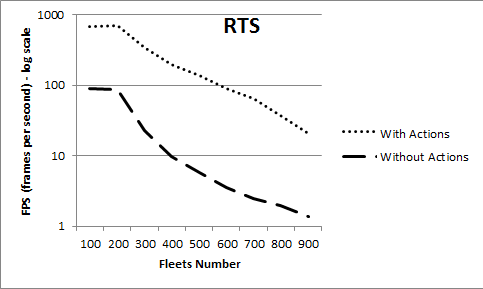
\includegraphics[height=5cm]{../RTS.png}
\end{frame}

\begin{frame}{Evaluation}
\center
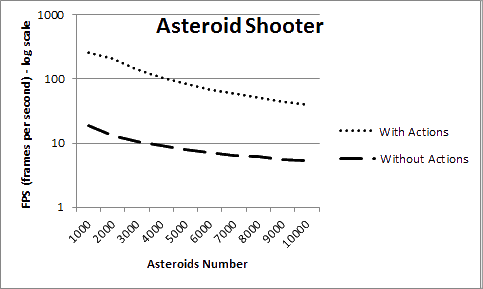
\includegraphics[height=5cm]{../Shooter.png}
\end{frame}

\begin{slide}{Evaluation}{Beyond RTS games}{
\item Also works for other kinds of games
\begin{itemize}
\item Shooters
\item RPGs
\item Pac-Man
\item Tetris
\item ...
\end{itemize}
}\end{slide}

\section{Closing}
\begin{slide}{Closing}{Discussion}{
\item We set out with the goal of reducing development effort for RTS games
\item The results are:
\begin{itemize}
\item Shorter, simpler sources
\item Significantly faster execution, without hand-made optimizations
\end{itemize}
\item We have built a well working prototype of Casanova embedded in F\#
}\end{slide}

\begin{slide}{Closing}{Future work}{
\item We are currently working on Casanova 2.0
\item Syntactic and semantic integration of rules, coroutines, and SQL
\begin{itemize}
\item Everything is done with rules
\item Every expression can interrupt, \texttt{yield} or \texttt{wait}
\item SQL is a first class expression
\item SQL queries are optimized with automated indices on \texttt{joins} and similar ``hotspots''
\end{itemize}
}\end{slide}

\begin{frame}{That's it!}
\begin{block}{Thank you!}
Questions?
\end{block}
\end{frame}

\end{document}
